\documentclass[answers]{exam}

\usepackage[a4paper,margin=2cm]{geometry}
%% Useful packages
\usepackage{amsmath}
\usepackage{graphicx}
\usepackage{paralist}
\usepackage{framed}
\usepackage{hyperref}


\setlength\FrameSep{4pt}
\title{CS 363 (Networks, Games, and Collective Behavior)\\ Homework - 01}
\author{Samarah Asghar Sahto, ss05563 \\ Zoha Ovais Karim, zk05617}
\date{28 February 2022}
\begin{document}
\maketitle

\noindent \hrulefill
\begin{questions}
    
    \question Q.1. [10 points] Consider an Erdös-Renyi (E-R) random network $G(n, p)$, where the $n=10^{9}$ and $p=10^{-5}$.
a) [01 point] Calculate the expected number of links $<m>$ generated from the above configuration of the above E-R network.\\
b) [01 point] Calculate the average degree $<k>$ of the above network.\\
c) [03 points] Calculate the probability that a randomly chosen node from the above E-R network has a degree $k=10^{5}$.\\
d) [02 points] What is the average path length of the above E-R network?\\
e) [03 points] Is the above E-R network expected to have all the nodes as part of one giant component? Justify your answer.
\begin{framed}
\textbf{Ans:} (a) $G(n.p)$
\\ $n=10^9$, $p=10^{-5}$\\ $<m>={n \choose 2}.p$=${10^9 \choose 2}*10^{-5}$ = $4.999 * 10^{12} \\ \approx 5 * 10^{12}$\\\\
(b) Avg. degree of a network is $<k>=\frac{\Sigma_{u \in V}deg(u)}{n}$\\where $\Sigma_{u \in V}deg(u)$ =2m (from Handshaking Lemma)\\$<k>=\frac{2<m>}{n}$=$<k>=(n-1).p$\\$<k>=(10^9 -1). 10 ^{-5}$\\=9999.99999\\ $\approx$ 10000 (Ans)\\\\
(c)$p_k=\frac{<k>^k.e^{-<k>}}{k!}$\\=$\frac{10000^{10^5}e^{(-10000)}}{10^5!}$\\=$\frac{infinity.0}{infinity}$\\$\approx$0\\from poisson dist, $p_k -> 0$\\\\
(d) apl= $\frac{ln(n)}{ln<k>}$\\$\frac{ln(10^9)}{ln(10000)}$\\=2.25\\\\(e) We saw in the Netlogo simulation how the E-R network works. The average degree is $<k>=(n-1) \cdot p$. In E-R random networks, all smaller components get absorbed into a single giant component when $<k> > ln(n)$ which is true in the case over here. 

\end{framed}

\question Q.2. [10 points] In the class, we discussed homophily in detail. Suppose, people in a society are divided into two distinct groups based on some social category (e.g., ethnicity), and data is collected about people's friends to construct a friendship network.
Let $\boldsymbol{n}{\mathbf{1}}$ be the size of group 1 and $\boldsymbol{n}{2}$ be the size of group 2. Also, assume $\boldsymbol{n}{\mathbf{1}}>\boldsymbol{n}{\mathbf{2}}$. We define a homophily metric for a group $\boldsymbol{g}$ as follows:
$$
\boldsymbol{h}{g}=\frac{\sum{i} s_{i}}{\sum_{i} d_{i}}
$$
where,
$\boldsymbol{s}{\boldsymbol{i}}$ is the number of friends that a person (node) $\boldsymbol{i}$ has from within its own group, and $\boldsymbol{d}{\boldsymbol{i}}$ is the total number of friends that a person (node) $\boldsymbol{i}$ has, i.e., degree of node $\boldsymbol{i}$.
Let $\boldsymbol{h}{1}$ and $\boldsymbol{h}{2}$ refer to the homophily metric for group 1 and group 2 respectively.
Show that if the average degree (average number of friends) of both the groups is about the same, and both $\boldsymbol{h}{1}$ and $\boldsymbol{h}{2}$ are greater than 0 and less than 1 , then $\boldsymbol{h}{1}>\boldsymbol{h}{2}$.

\begin{framed}
\textbf{Ans:} We know that there exists two groups, $n1$ and $n2$. Moreover, $n1 > n2$ which means more number of nodes in group than in group 2. \\ The formula for the homophily metric has been given. \\ It is also mentioned that the average degree of nodes in both groups is about the same. This leads us to two assumptions. Avg. degree of group 1 can be as high as the average degree in group 2. For example, the average degree of a node i in group 1 is same as the average degree of node j in group 2. This is the denominator in the metric. Let us take the average degree to be $k$. $k$ is the sum of degrees of node i in group 1 and group 2. $k$=deg(group1)+deg(group2).\\
$h_1=\frac{\Sigma_i(s_i)}{k}$\\
$h_2=\frac{\Sigma_j(s_j)}{k}$ \\
$\Sigma_i(s_i)$=$k$-deg(group2)\\
$\Sigma_j(s_j)$=$k$-deg(group1)\\
Similarly, the second case can also be true in which the average degree for a node in group 1 is higher than that of a node in group 2. However,
from the concept of homophily we know, \\ A research paper called A Simple Model of Homophily in Social Networks explains homophily as follows, 'A pervasive feature of social and economic networks is that contacts tend to be more frequent
among similar agents than among dissimilar ones. This pattern, usually referred to as “homophily”,
applies to many types of social interaction, and along many dimensions of similarity.'\\ People tend to be in groups with people of similar habits. Since group 1 is larger, a node in group 1 will have more connections as more nodes present and it is likely to form links with most of those nodes because of the idea of homophily (similar thinking). In both cases, the ratio of group 1 is to be larger. Since it is a homophily metric, we can assume that the connections are denser because a node is very likely to be forming links with most nodes in its group because of similar-mindedness and similar habits. One group will have people with similar mindsets hence assuming that the node is connected to most of the nodes. Thus, the numerator for the group 1 metric would be larger than the numerator for the group 2 metric and so is the case with the denominator, therefore the ratio for group 1 is larger than ratio of group 2. So $h1 > h2$, shown. \\

\end{framed}

    \question [10 points] Consider a regular ring lattice network where each node has six $(06)$ connections. What will be the average clustering coefficient of this network? [Hint: Use the Home Reading shared in the module for Week 07].
    
\begin{framed}
\newpage
\textbf{Ans:} 
The graph given to us is a regular ring lattice with $k=6$.\\
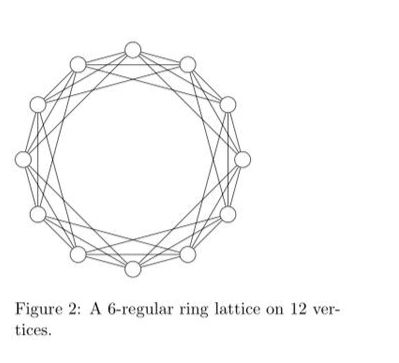
\includegraphics[width=10cm]{q3.jpeg}\\
The local clustering coefficient gives us the average clustering coefficient. Now, as we also did in class following the same procedure of local clustering coefficient:
\begin{center}
    $\frac{2 * L_i}{k(k-1)}$ where $L_i$ = no. of neighbours of neighbours\\
    $\frac{2*9}{6(5)} = 0.6$
\end{center}





\end{framed}

\question Q.4. [20 points] Programming Exercise $^{1}$. Submit the GitHub link for your solution, which should contain the source code, datasets generated, and any other relevant material).

Write a program to generate an Erdös-Renyi (E-R) network $G(n, p)$, were for at least three input configurations, i.e., three set of values for $n$ and $p$. For instance, one such configuration could be $n=7 * 10^{6}$ and $p=10^{-2}$. For each configuration, calculate the following network properties and compare them with the theoretical prediction for an Erdös-Renyi network with the same configuration. Run each configuration at least 30 times and report the average estimates for each configuration.\\
i. The average degree of the network.\\
ii. Average clustering coefficient of the network.\\
iii. The average path length.\\
iv. Plot the degree distribution for the three chosen configurations. Do they center on the average degree?\\

(10 points for implementation with sharing of a working code; 15 points for calculations i, ii, and iii; 15 points for the plots of degree distributions.)

\begin{framed}

\textbf{Ans:} Github Link for this question:   \textbf{\url{https://github.com/zoha99/Networks-Homework-2}}\\
First configuration, $n=3*10^6$, $p=0.25$\\Second Configuration, $n=10*10^3$, $p=0.1$ \\Third Configuration, $n=6*10^6$, $p=0.08$\\\\We made use of the networkx package on python to generate Erdos Renyi Networks using the three configurations mentioned above. The code was run 30 times for each configuration and the networks obtained were as follows:
\\\\
Configuration 1:\\Network when I run for the rth time, r=1:\\
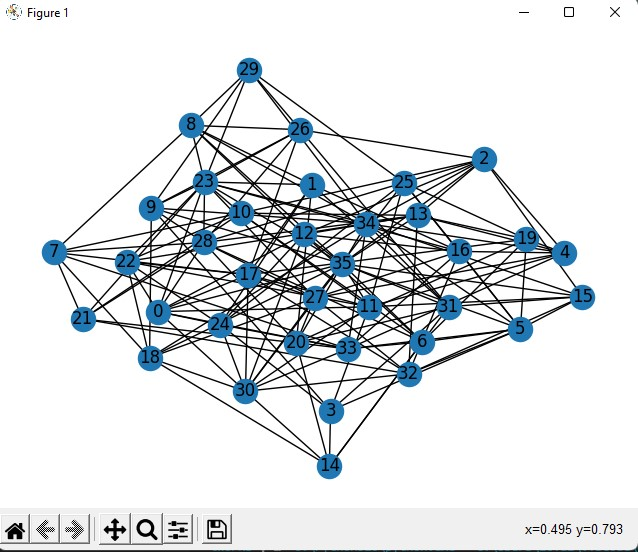
\includegraphics[width=10 cm]{first conf 1.jpg}\\

r=10:\\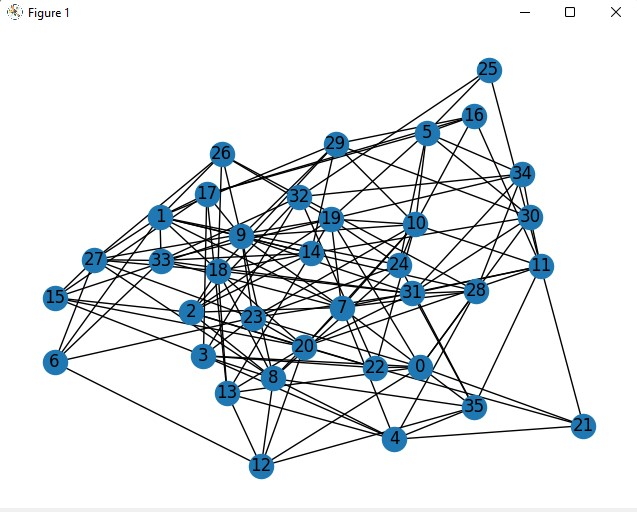
\includegraphics[width=10 cm]{first conf 10.jpg}\\
r=20:\\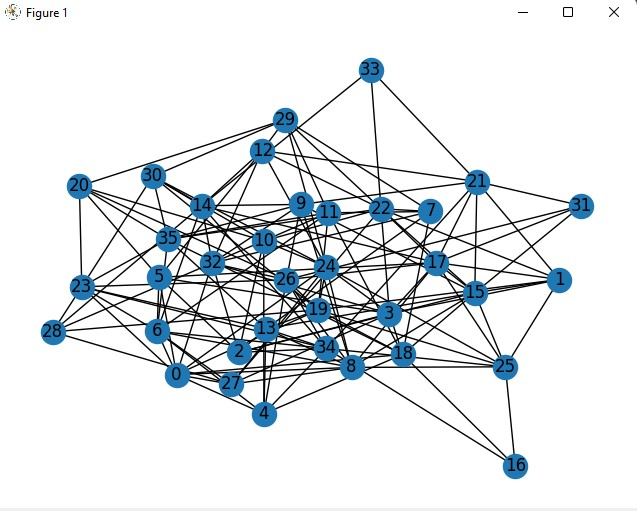
\includegraphics[width=10 cm]{first conf 20.jpg}\\
r=30:\\ 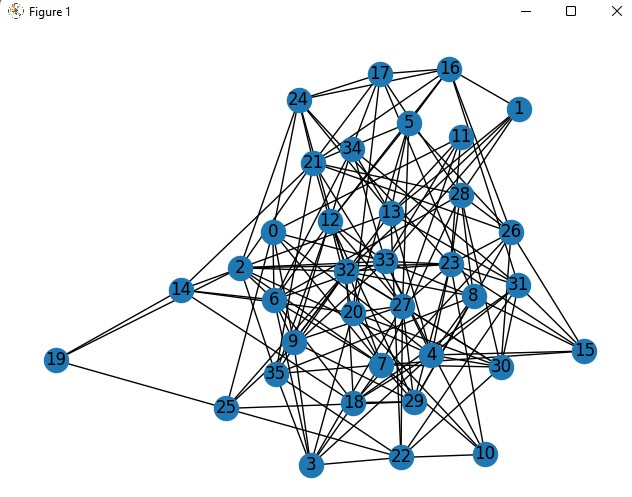
\includegraphics[width=10 cm]{first conf 30.jpg}\\\\
Configuration 2:\\Network when I run for the rth time, r=1:\\
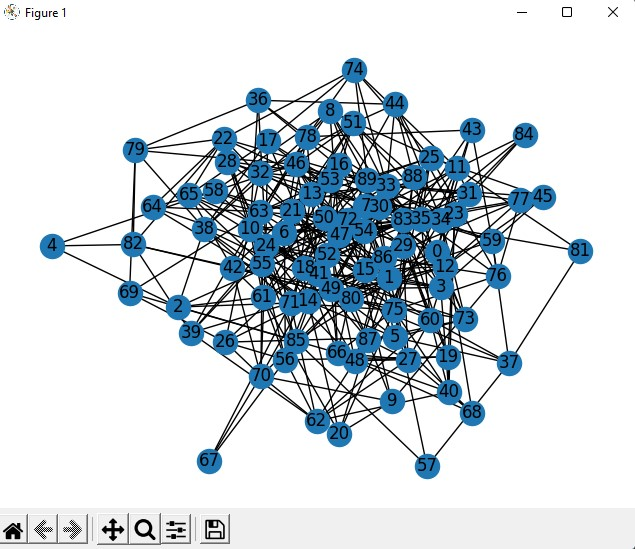
\includegraphics[width=10 cm]{sec conf pic 1.jpg}\\

r=10:\\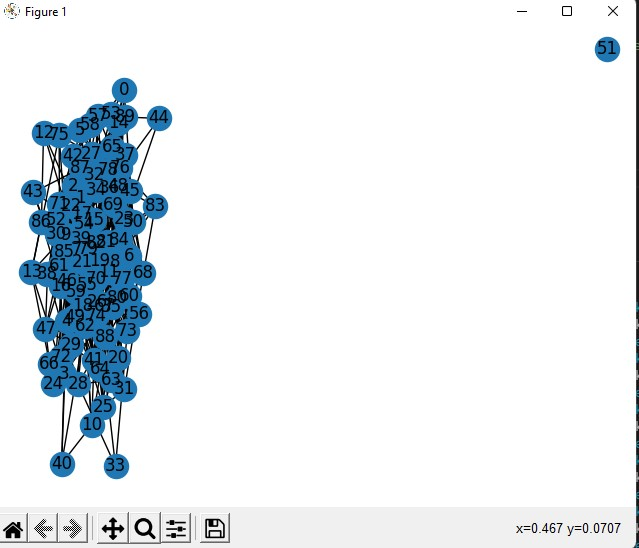
\includegraphics[width=10 cm]{sec conf10th.jpg}\\r=20:\\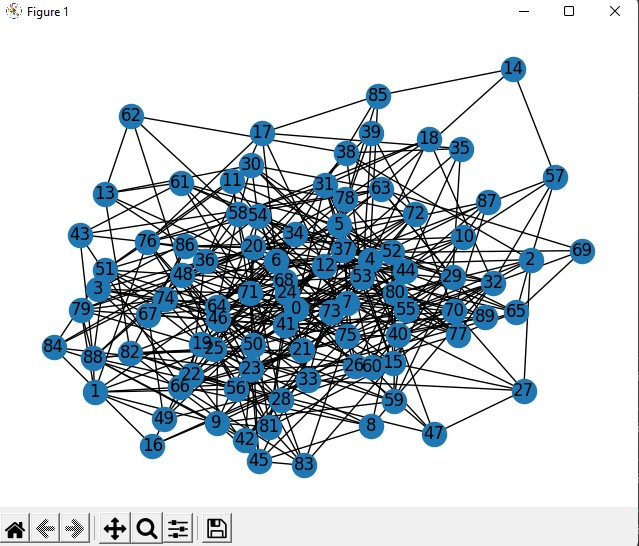
\includegraphics[width=10 cm]{20th sec conf.jpg}\\r=30:\\ 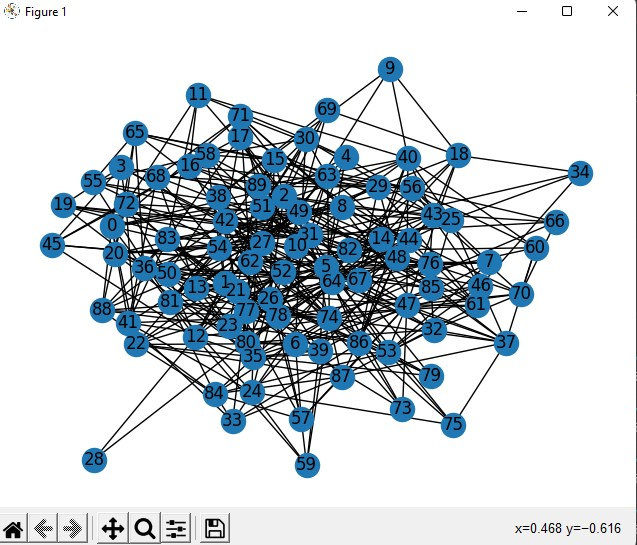
\includegraphics[width=10 cm]{30th sec conf.jpg}\\\\
Configuration 3:\\Network when I run for the rth time, r=1:\\
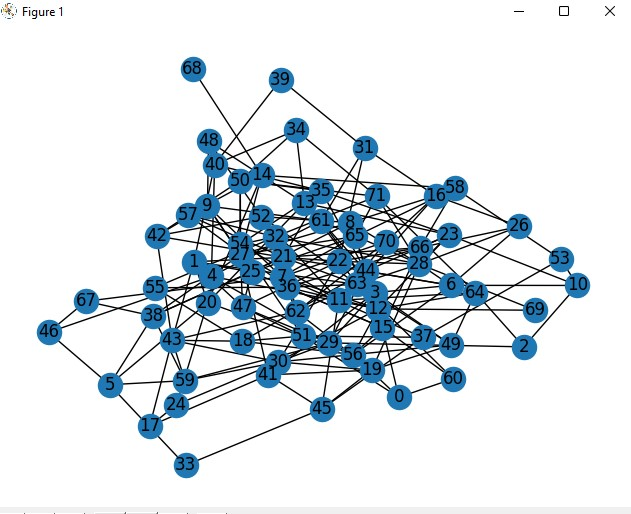
\includegraphics[width=10 cm]{3rd conf 1.jpg}

r=10:\\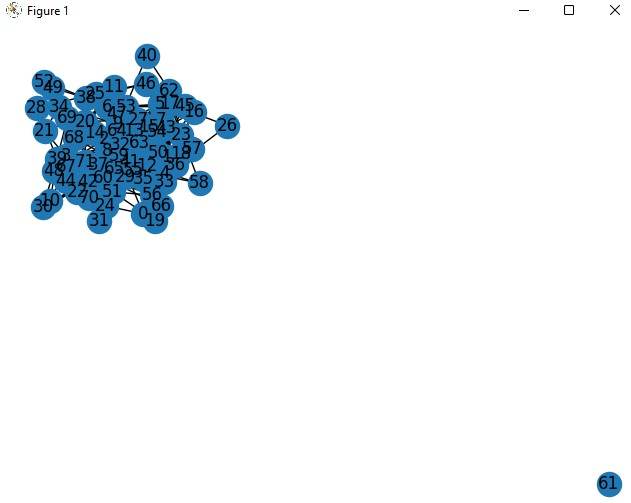
\includegraphics[width=10 cm]{3rd conf 10.jpg}\\
r=20:\\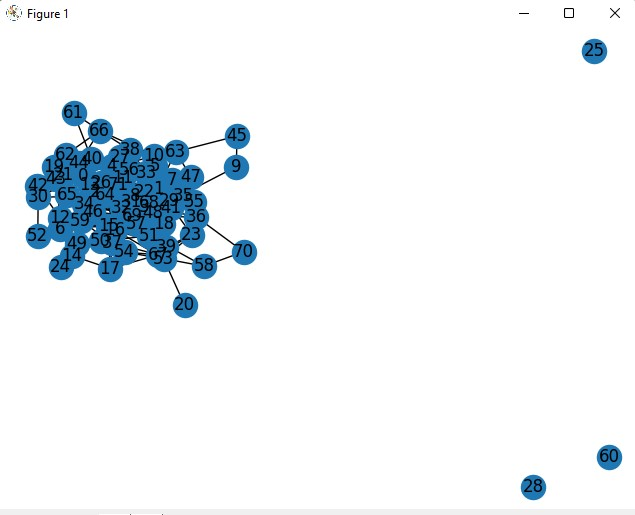
\includegraphics[width=10 cm]{3rd conf 20.jpg}\\
r=30:\\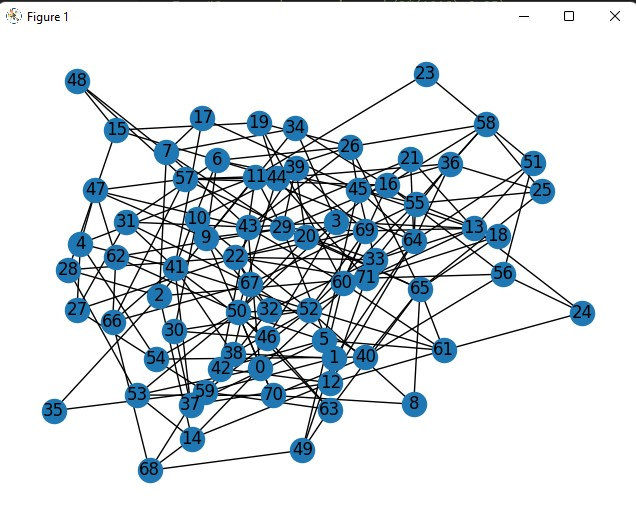
\includegraphics[width=10 cm]{3rd conf 30.jpg}\\

First configuration, $n=3*10^6$, $p=0.25$\\$i)$ avg. degree =(n-1)$\cdot$p = 749999.75\\
$ii)$ Using the built-in function of networkx, $nx.average\_clustering(G)$, for this configuration $G$, the average clustering coefficient obtained is: 0.253\\ 
Theoretically, the expected local clustering coefficient = p = 0.25 and it is seen in the respective Average Clustering Histogram that on average the clustering coefficient is mostly near the p value.\\
\\$iii)$ $apl=\frac{ln(n)}{ln<k>}$=$\frac{ln(3*10^6)}{ln(749999.75)}$\\=1.102\\\\
Second Configuration, $n=10*10^3$, $p=0.1$ \\ $i)$ avg.degree=(n-1)$\cdot$p \\= 999.9 \\
$ii)$ Using the built-in function of networkx, $nx.average\_clustering(G)$, for this configuration $G$, the average clustering coefficient obtained is: 0.104\\ Theoretically, the expected local clustering coefficient = p = 0.1 and it is seen in the respective Average Clustering Histogram that on average the clustering coefficient is mostly near the p value.
\\ $iii)$ $apl=\frac{ln(n)}{ln<k>}$= $\frac{ln(10*10^3)}{ln(999.9)}$\\=1.33\\\\
Third Configuration, $n=6*10^6$, $p=0.08$\\$i)$ avg.degree=(n-1)$\cdot$p \\= 479999.92\\
$ii)$ Using the built-in function of networkx, $nx.average\_clustering(G)$, for this configuration $G$, the average clustering coefficient obtained is: 0.0796\\ Theoretically, the expected local clustering coefficient = p = 0.08 and it is seen in the respective Average Clustering Histogram that on average the clustering coefficient is mostly near the p value.
\\$iii)$ $apl=\frac{ln(n)}{ln<k>}$=$\frac{ln(6*10^6)}{ln(479999.92)}$\\=1.19\\\\
For all parts $i,ii,iii$, (code included in the github link), we have generated histograms running the loop 30 times in order to get the plots for all three properties of the network for all three configurations.
\newpage
\textbf{First configuration, $n=3*10^6$, $p=0.25$:}\\
\textbf{Average Degree Histogram:} \\ 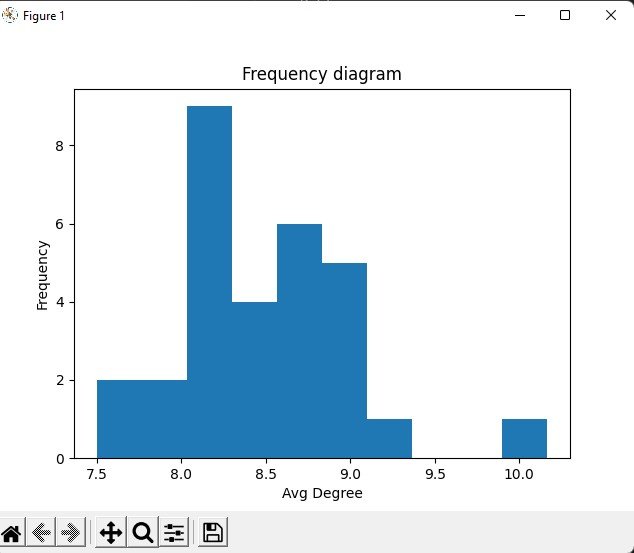
\includegraphics[width=10cm]{G1 avg degree.jpg}\\
\textbf{Average Clustering Histogram:}\\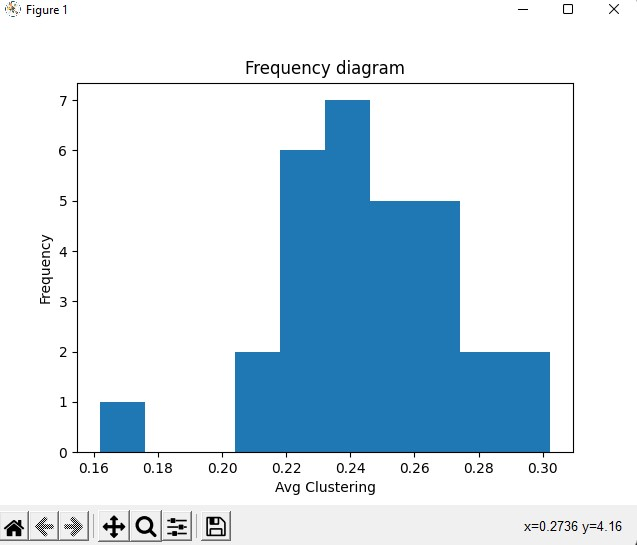
\includegraphics[width=10cm]{Average Clustering 1.jpg}
\newpage
\textbf{Average Path Length Histogram:}\\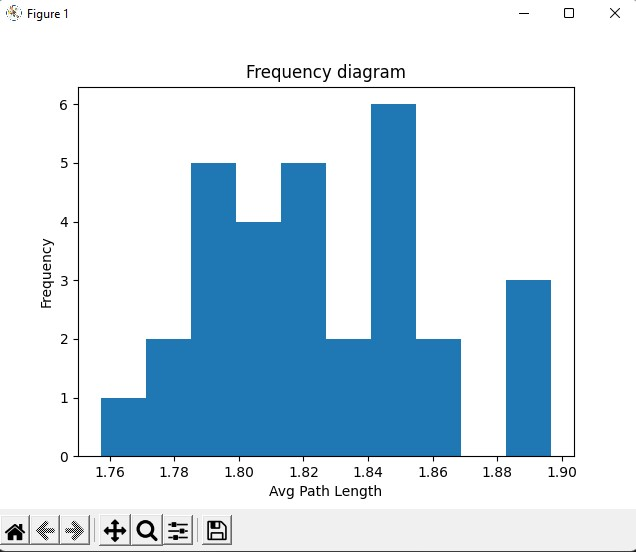
\includegraphics[width=10cm]{Average Path Length.jpg}\\\\\textbf{$iv) $Degree Distribution Plot}\\ 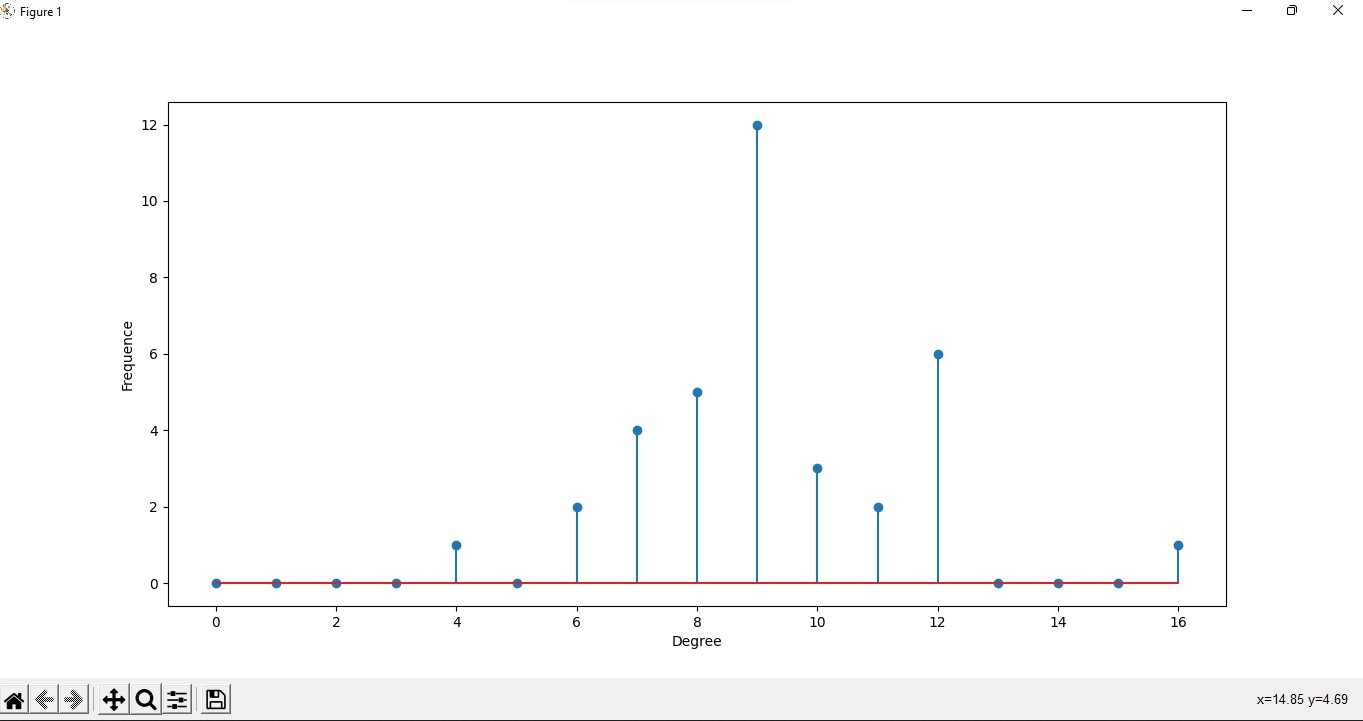
\includegraphics[width=10cm]{deg distribution 1.jpg}\\\\
\newline
\textbf{Second Configuration,$n=10*10^3$, $p=0.1$:} \\\textbf{Average Degree Histogram:} \\ 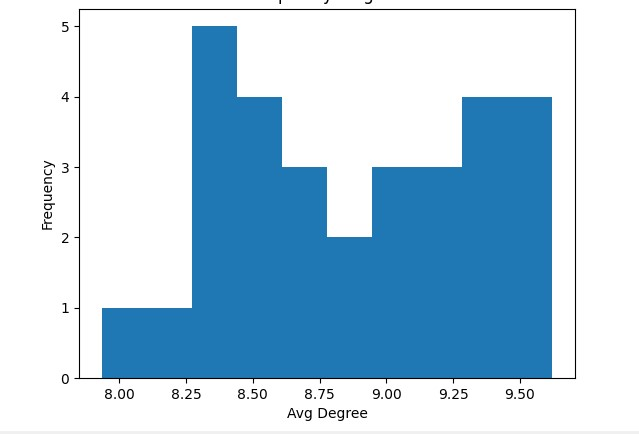
\includegraphics[width=10cm]{avg degree 2.jpg}\\
\newpage
\textbf{Average Clustering Histogram:}\\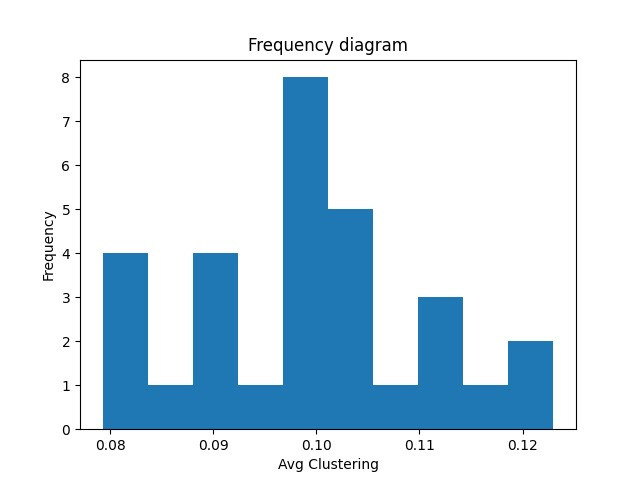
\includegraphics[width=10cm]{g2-cc.jpg}\\\textbf{Average Path Length Histogram:}\\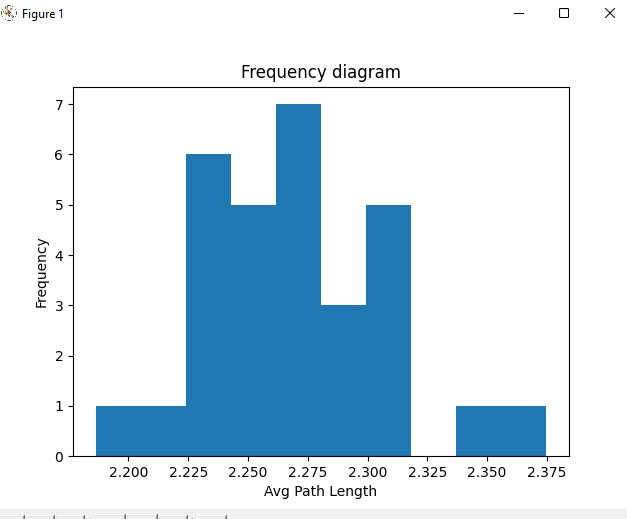
\includegraphics[width=10cm]{apl 2.jpg}\\\\\textbf{$iv) $ Degree Distribution Plot:}\\ 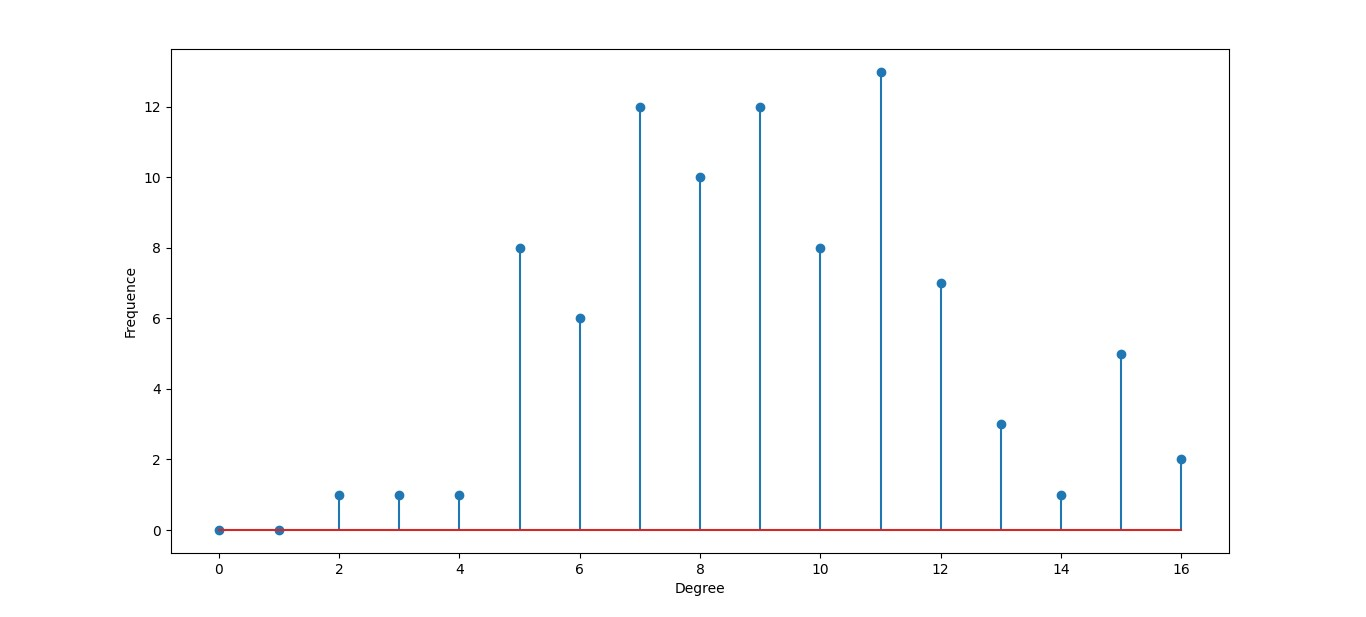
\includegraphics[width=10cm]{deg dist 2.jpg}\\\\
\newpage
\textbf{Third Configuration, $n=6*10^6$, $p=0.08$:}\\\textbf{Average Degree Histogram:} \\ 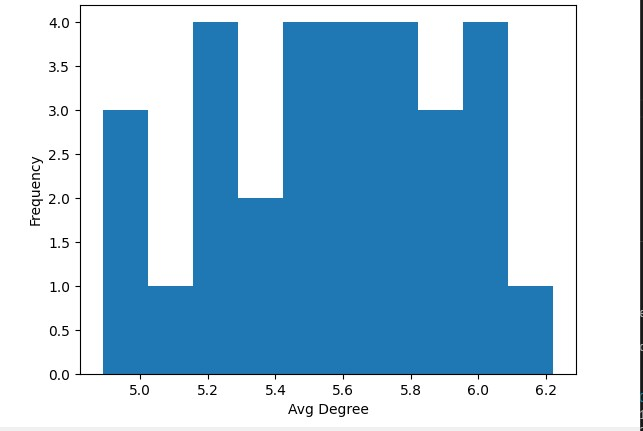
\includegraphics[width=10cm]{avg degree 3.jpg}\\\textbf{Average Clustering Histogram:}\\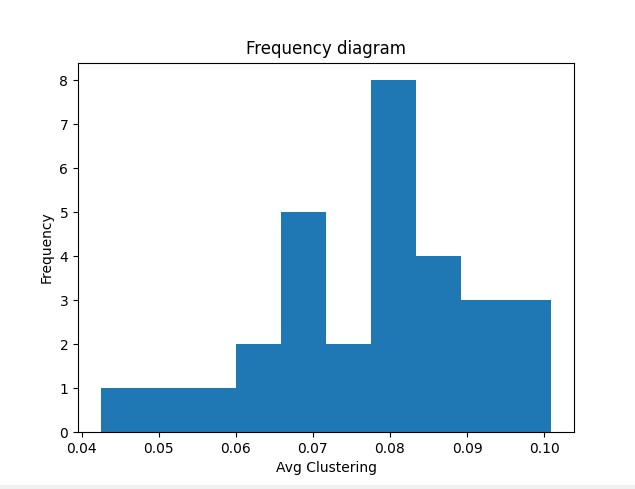
\includegraphics[width=10cm]{g3-cc.jpg}\\\textbf{Average Path Length Histogram} Under this configuration, we did not obtain the histogram for the average path length because the graph is unconnected and it raises an error in generating the average for 30 simulations. We can also notice this in the simulation snapshots attached for Configuration 3. \\\\\textbf{$iv) $Degree Distribution Plot} \\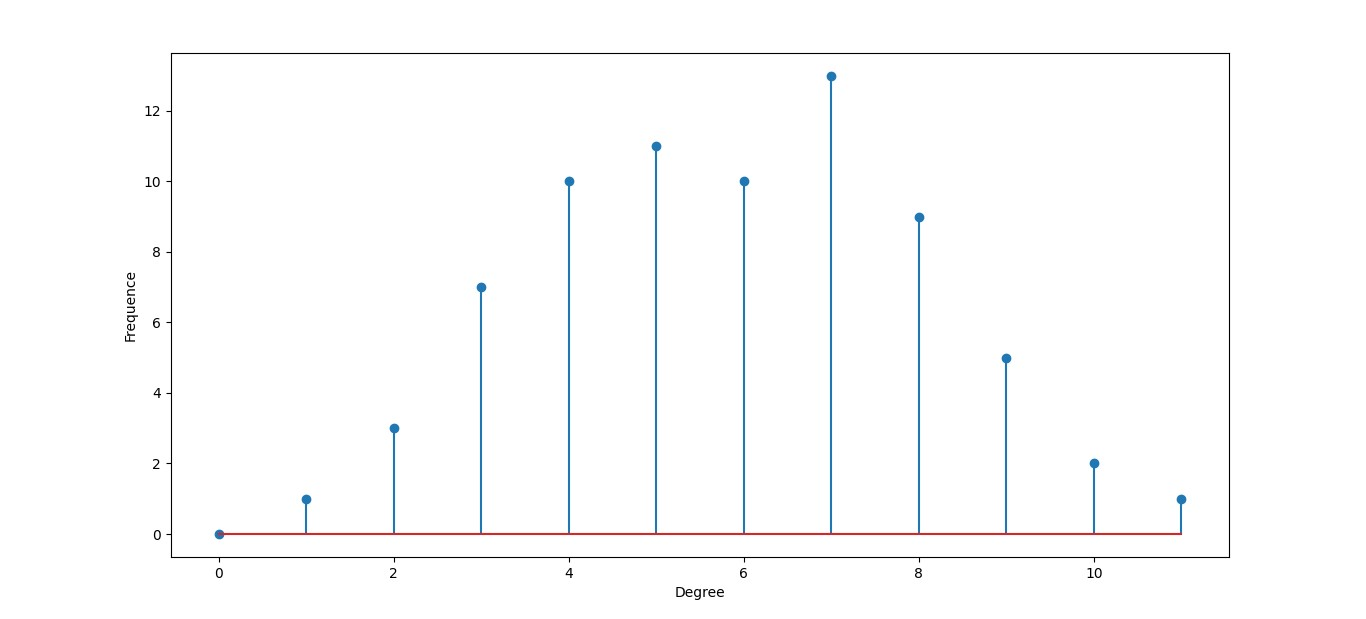
\includegraphics[width=10cm]{deg dist 3.jpg}
\\\\The three properties of the network are close to our theoretical calculations. The Average Degree that we obtain in our histogram is a value a little greater than the original value that we got however, the difference in the calculated value and the graphical average degree is not a huge difference. The average degree in the histogram is dense around the calculated values that we obtained.\\


The expected local clustering value theoretically equals to the value of $p$, and this is what we also notice that the histogram gives a gathered or dense plot around the value of $p$ making it the average clustering coefficient. For instance the value of $p$ for the first configuration is 0.25 and the histogram plot also gives the same result as we can see the highest bar around that value.\\
For the average path length, the values that we obtained via calculations and what we got via our histogram representation are a little different. However, it is justified  because the built in networkx function that we are using to calculate the average path length is not using the same theoretical formula that we use involving natural log. The built in function, $nx.average\_shortest\_path\_length(G))$ is making use of the formula below:\\ $\sum_{s,t \in V} 
\frac{d(s,t)}{n(n-1)}$ where V is the set of nodes in G, d(s, t) is the shortest path from s to t, and n is the number of nodes in G. \\The degree distribution plots are all in line with the theoretical concept of the Erdos Renyi Networks as it gives us a Poisson Distribution graph representation. 
\end{framed}

\end{questions}
\begin{thebibliography}{9}
\bibitem   . Question 1: CS-363 Handwritten Notes \\CS 363- Week 04 Slides 
\bibitem   . Question 2: \url{https://eprints.whiterose.ac.uk/137644/1/currarini_matheson_redondo_2016.pdf}

\bibitem   . Question 3:
\url{https://people.seas.harvard.edu/~yaron/cs284r/1-sep4.pdf}

\bibitem   . Question 4:
\url{https://www.geeksforgeeks.org/implementation-of-erdos-renyi-model-on-social-networks/}\\
\url{https://networkx.org/documentation/networkx-1.10/reference/generated/networkx.algorithms.shortest_paths.generic.average_shortest_path_length.html}\\ \url{https://networkx.org/documentation/networkx-0.37/}



  \end{thebibliography}
  
\end{document}